%        File: report.tex
%     Created: Thu May 04 03:00 PM 2017 A
% Last Change: Thu May 04 03:00 PM 2017 A
%
\documentclass[conference, a4paper]{IEEEtran}

\usepackage{cite, graphicx, amsmath} 
\interdisplaylinepenalty=2500

% *** Do not adjust lengths that control margins, column widths, etc. ***
% *** Do not use packages that alter fonts (such as pslatex).         ***
% There should be no need to do such things with IEEEtran.cls V1.6 and later.


% correct bad hyphenation here
%\hyphenation{<+op-tical net-works semi-conduc-tor+>}


\begin{document}
%
% paper title
\title{Conceptual Design of a Real-Time Pedicle Screw Positioning Sensor for
Spinal Surgery}
\author{Luke Warlik and Gareth Arnold}


% make the title area
\maketitle


\begin{abstract}
	<+The abstract goes here.+>
\end{abstract}


\section{Introduction}
This demo file is meant to serve as a starter file for the
IEEEtran latex template maybe I need more text here how about this
I'll just keep typing and maybe the error will go away
% You must have at least 2 lines in the paragraph with the drop letter
% (should never be an issue)
<+May all your publication endeavors be successful.+>

\section{Ultrasonics Image Guidance}
Ultrasound is an imaging technique that involves emmiting sound waves into a
body. The sound waves are above the limit of human hearing, often being in
the order of mHz. An image is created by capturing the waves reflected
by the organs in the body. 
The process relies on the fact that the sound will interact with
different areas of the body differently depending on their density and
structure. A common use for ultrasonic imaging is obstetric ultrasound,
the process of examining the wombs of pregnant women. 

Ultrasound has several advantages over other types of imaging, including:
being non-invasive, safe and relatively painless, not using ionising radiation,
not requiring an injection of a contrast medium and being able to be used in
many different areas of the body\cite{imagingExplained}. Of special interest
in the case of a 
pedicle screw operation is the use of sound instead of ionising radiation,
as the patient and surgeon will not be exposed to the risks of ionising
radiation. 

The current method for inserting pedicle screws is as follows: 
Firstly a small inciscion is created in the patient's back close to the area
where the screw will be placed. Then the surgeon uses an bone awl tool
to puncture a hole in the outside layer of the bone, before working the
sharp tip of the tool through the soft inner part of the bone. The surgeon
relies on previous experience of the resistance of different types of bone to
determine the correct heading for the tool. Once the hole has been created,
either a smaller pedicle screw will be inserted to clear out and tap the hole
with an interference fit for a larger screw, or the full sized screw will be
inserted. The process is repeated on the other side of the vertebrae, and 
on at least one other vertebra. Metal rods are then used to lock the two screws
together and prevent the movement of the 2 bones. 

Bone is a rigid organ that developed to, among other things, 
provide structural support for the human body. It is made primarily of
collagen, is has two different macro level structures: Cortical and Canellous 
bone. The cortical bone makes up the exterior of the bone, and is a hard, 
densely packed structure. Canellous bone, on the other hand, makes up the
interior of the bone, and appears porous and sponge like. These structures
can be seen in Figure \ref{fig:boneStruct}.

\begin{figure}
	\centering
	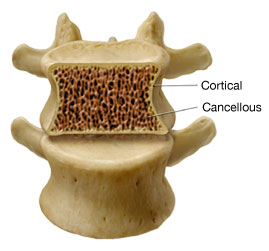
\includegraphics{assets/boneStruct.jpg}
	\caption{Cortical and Cancellous bone structures \cite{boneStructure}}
	\label{fig:boneStruct}
\end{figure}

As stated previously, surgeons have traditionally relied on their own
experience of the feeling of the different structures of bones while
making the hole for the screw drilling. Samdani et al \cite{Samdani2010}
investigated whether the accuracy of a surgeon while placing pedicle screws
was related to their experience. It was found that there was no statistical
significance (p=0.58) between the groups of surgeons with differenct 
experience levels. This suggests that a more accurate method for determining
accuracy while placing pedicle screws is required.

As discussed previously,
differences between the structures of the 2 different components of bones
provide a way with which the accuracy of the placement of a pedicle screw hole
can be measured in real time. The proposed method is to use an ultrasonic 
sensor to determine the differences in density between to two bone structures
in the hope that the accuracy of the hole trajectory can be determined by the
surgeon in real time without line of sight on the operating area. 





% trigger a \newpage just before the given reference
% number - used to balance the columns on the last page
% adjust value as needed - may need to be readjusted if
% the document is modified later
%\IEEEtriggeratref{8}
% The "triggered" command can be changed if desired:
%\IEEEtriggercmd{\enlargethispage{-5in}}

% references section

%\bibliographystyle{IEEEtran.bst}
%\bibliography{IEEEabrv,../bib/paper}

\bibliography{report}
\bibliographystyle{IEEEtran}

% insert where needed to balance the two columns on the last page
%\newpage


\end{document}



